% Generated 2021-08-25 18:02:25 +0530
\subsection{CuttingItem Measurement Types} \label{sec:CuttingItem Measurement Types}


This section lists the \block{Measurement} types for \block{CuttingItem}.

will be used to for reference for the \block{CuttingItem} specific \block{Measurement} types.

\begin{figure}[ht]
  \centering
    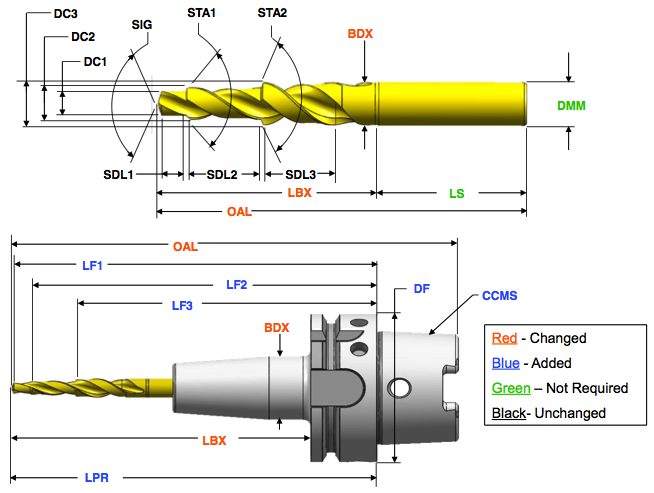
\includegraphics[width=1.0\textwidth]{figures/Cutting Tool.png}
  \caption{Cutting Tool Diagram}
  \label{fig:Cutting Tool Diagram}
\end{figure}

\FloatBarrier


\begin{figure}[ht]
  \centering
    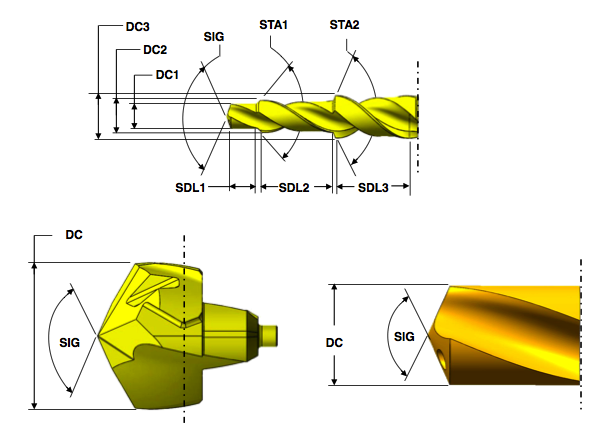
\includegraphics[width=1.0\textwidth]{figures/Cutting Item.png}
  \caption{Cutting Item Diagram}
  \label{fig:Cutting Item Diagram}
\end{figure}

\FloatBarrier


\begin{figure}[ht]
  \centering
    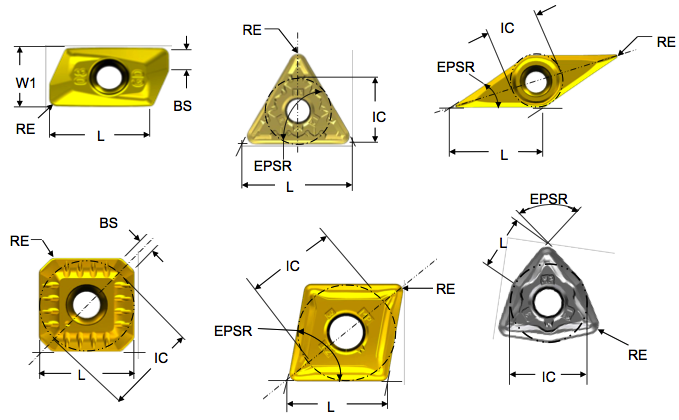
\includegraphics[width=1.0\textwidth]{figures/Cutting Item Measurement.png}
  \caption{Cutting Item Measurement Diagram}
  \label{fig:Cutting Item Measurement Diagram}
\end{figure}

\FloatBarrier


\begin{figure}[ht]
  \centering
    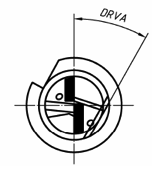
\includegraphics[width=1.0\textwidth]{figures/Cutting Item Drive Angle.png}
  \caption{Cutting Item Drive Angle Diagram}
  \label{fig:Cutting Item Drive Angle Diagram}
\end{figure}

\FloatBarrier



\subsubsection{ChamferFlatLength}
\label{sec:ChamferFlatLength}



The flat length of a chamfer.


\texttt{code}: \texttt{BCH}.


\texttt{units}: \texttt{MILLIMETER}.



\subsubsection{ChamferWidth}
\label{sec:ChamferWidth}



The width of the chamfer.


\texttt{code}: \texttt{CHW}.


\texttt{units}: \texttt{MILLIMETER}.



\subsubsection{CornerRadius}
\label{sec:CornerRadius}



The nominal radius of a rounded corner measured in the X Y-plane.


\texttt{code}: \texttt{RE}.


\texttt{units}: \texttt{MILLIMETER}.



\subsubsection{CuttingDiameter}
\label{sec:CuttingDiameter}



The diameter of a circle on which the defined point Pk located on this Cutting Tool. The normal of the machined peripheral surface points towards the axis of the Cutting Tool.


\texttt{code}: \texttt{DCx}.


\texttt{units}: \texttt{MILLIMETER}.



\subsubsection{CuttingEdgeLength}
\label{sec:CuttingEdgeLength}



The theoretical length of the cutting edge of a Cutting Item over sharp corners.


\texttt{code}: \texttt{L}.


\texttt{units}: \texttt{MILLIMETER}.



\subsubsection{CuttingHeight}
\label{sec:CuttingHeight}



The distance from the basal plane of the Tool Item to the cutting point.


\texttt{code}: \texttt{HF}.


\texttt{units}: \texttt{MILLIMETER}.



\subsubsection{CuttingReferencePoint}
\label{sec:CuttingReferencePoint}



The theoretical sharp point of the Cutting Tool from which the major functional dimensions are taken.


\texttt{code}: \texttt{CRP}.


\texttt{units}: \texttt{MILLIMETER}.



\subsubsection{DriveAngle}
\label{sec:DriveAngle}



Angle between the driving mechanism locator on a Tool Item and the main cutting edge.


\texttt{code}: \texttt{DRVA}.


\texttt{units}: \texttt{DEGREE}.



\subsubsection{FlangeDiameter}
\label{sec:FlangeDiameter}



The dimension between two parallel tangents on the outside edge of a flange.


\texttt{code}: \texttt{DF}.


\texttt{units}: \texttt{MILLIMETER}.



\subsubsection{FunctionalLength}




The distance from the gauge plane or from the end of the shank of the Cutting Tool, if a gauge plane does not exist, to the cutting reference point determined by the main function of the tool. This measurement will be with reference to the Cutting Tool and \textbf{MUSTNOT} exist without a Cutting Tool.


\texttt{code}: \texttt{LFx}.


\texttt{units}: \texttt{MILLIMETER}.



\subsubsection{FunctionalWidth}
\label{sec:FunctionalWidth}



The distance between the cutting reference point and the rear backing surface of a turning tool or the axis of a boring bar.


\texttt{code}: \texttt{WF}.


\texttt{units}: \texttt{MILLIMETER}.



\subsubsection{IncribedCircleDiameter}
\label{sec:IncribedCircleDiameter}



The diameter of a circle to which all edges of a equilateral and round regular insert are tangential.


\texttt{code}: \texttt{IC}.


\texttt{units}: \texttt{MILLIMETER}.



\subsubsection{InsertWidth}
\label{sec:InsertWidth}



W1 is used for the insert width when an inscribed circle diameter is not practical.


\texttt{code}: \texttt{W1}.


\texttt{units}: \texttt{MILLIMETER}.



\subsubsection{PointAngle}
\label{sec:PointAngle}



The angle between the major cutting edge and the same cutting edge rotated by 180 degrees about the tool axis.


\texttt{code}: \texttt{SIG}.


\texttt{units}: \texttt{DEGREE}.



\subsubsection{StepDiameterLength}
\label{sec:StepDiameterLength}



The length of a portion of a stepped tool that is related to a corresponding cutting diameter measured from the cutting reference point of that cutting diameter to the point on the next cutting edge at which the diameter starts to change.


\texttt{code}: \texttt{SDLx}.


\texttt{units}: \texttt{MILLIMETER}.



\subsubsection{StepIncludedAngle}
\label{sec:StepIncludedAngle}



The angle between a major edge on a step of a stepped tool and the same cutting edge rotated 180 degrees about its tool axis.


\texttt{code}: \texttt{STAx}.


\texttt{units}: \texttt{DEGREE}.



\subsubsection{ToolCuttingEdgeAngle}
\label{sec:ToolCuttingEdgeAngle}



The angle between the tool cutting edge plane and the tool feed plane measured in a plane parallel the xy-plane.


\texttt{code}: \texttt{KAPR}.


\texttt{units}: \texttt{DEGREE}.



\subsubsection{ToolLeadAngle}
\label{sec:ToolLeadAngle}



The angle between the tool cutting edge plane and a plane perpendicular to the tool feed plane measured in a plane parallel the xy-plane.


\texttt{code}: \texttt{PSIR}.


\texttt{units}: \texttt{DEGREE}.



\subsubsection{ToolOrientation}
\label{sec:ToolOrientation}



The angle of the tool with respect to the workpiece for a given process. The value is application specific.


\texttt{code}: \texttt{N/A}.


\texttt{units}: \texttt{DEGREE}.



\subsubsection{Weight}




The total weight of the Cutting Tool in grams. The force exerted by the mass of the Cutting Tool.


\texttt{code}: \texttt{WT}.


\texttt{units}: \texttt{GRAM}.



\subsubsection{WiperEdgeLength}
\label{sec:WiperEdgeLength}



The measure of the length of a wiper edge of a Cutting Item.


\texttt{code}: \texttt{BS}.


\texttt{units}: \texttt{MILLIMETER}.


